\documentclass{article}

\usepackage[italian]{babel}
\usepackage[letterpaper,top=2cm,bottom=2cm,left=3cm,right=3cm,marginparwidth=1.75cm]{geometry}
\usepackage{amsmath}
\usepackage{graphicx}
\usepackage{subcaption}
\usepackage{textcomp}
\usepackage{ragged2e}
\usepackage[dvipsnames]{xcolor}
\usepackage{fancyhdr}
\usepackage[colorlinks=true, allcolors=blue,
            pdfauthor={Matteo Drago},
            pdftitle={Bivacco Vigolana "alla Madonnina" o Giacomelli},
            pdfsubject={Diario bivacchi e trekking},
            pdfkeywords={bivacco, montagna, trekking, diario}]{hyperref}

\title{\textbf{Bivacco Vigolana “alla Madonnina” o Bivacco Giacomelli - 2030 m s.l.m}}
\author{Matteo Drago}

% ==========================================================
% Impostazioni per il logo in ogni pagina
% ==========================================================
\pagestyle{fancy}
\fancyhf{} % Pulisce tutti i campi di intestazione e piè di pagina
\fancyhead[R]{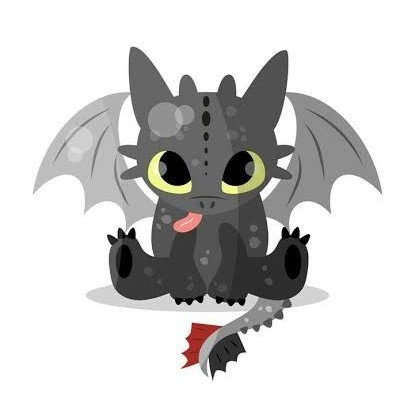
\includegraphics[height=1.5cm]{images/toothless.jpeg}} % Posiziona il logo a destra (R) nell'intestazione
\renewcommand{\headrulewidth}{0pt} % Rimuove la linea orizzontale nell'intestazione (opzionale)


\begin{document}
\maketitle
\thispagestyle{fancy} % Aggiungi questa riga

\begin{abstract}
Questo documento raccoglie e organizza le informazioni che ho acquisito nel corso degli anni sui bivacchi, basate sulle mie esperienze dirette. Sebbene non si proponga come una guida esaustiva e perfetta, offre il minimo indispensabile per una buona vita in bivacco, con consigli pratici e diretti per chiunque desideri affrontare al meglio queste pazze ma piacevoli avventure.
\end{abstract}

\section{Il bivacco}

% ==========================================================
% Immagine a sinistra, testo a destra allineato in alto
% ==========================================================
\noindent
\begin{minipage}[t]{0.45\textwidth}
  \vspace{0pt} % forza l'allineamento in alto
  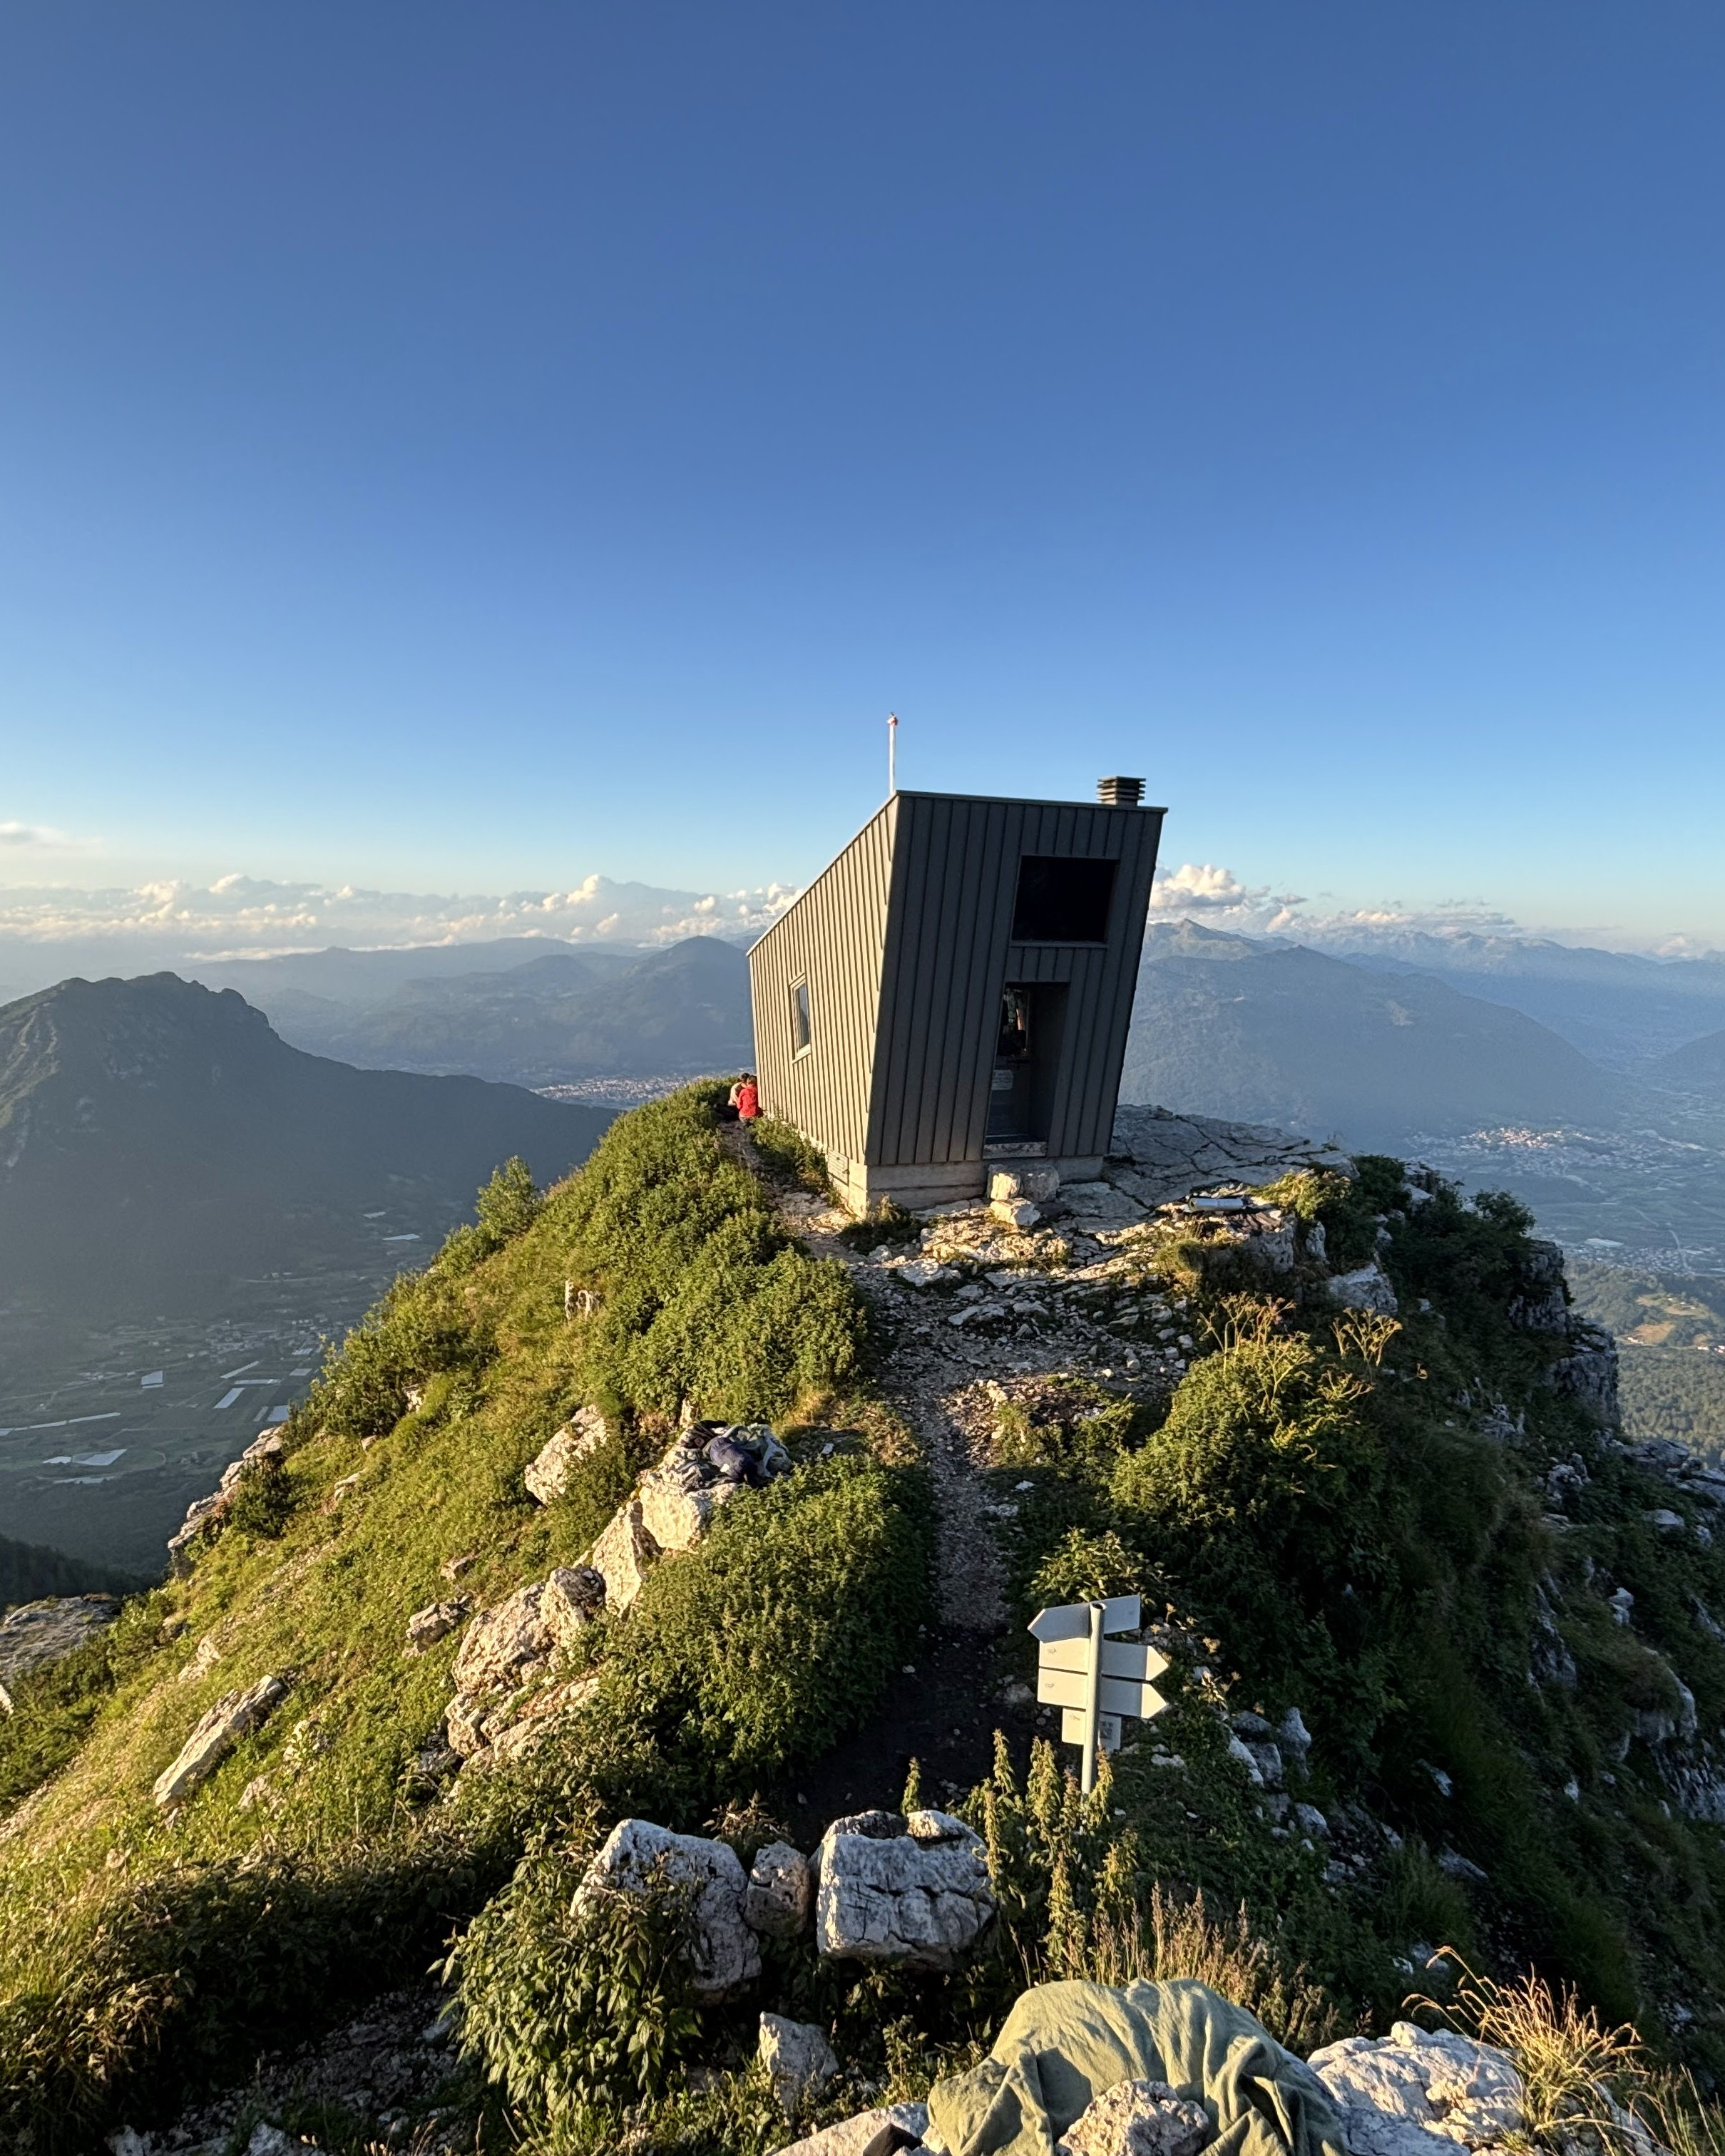
\includegraphics[width=\linewidth]{images/bivacco.jpg}
\end{minipage}%
\hfill
\begin{minipage}[t]{0.5\textwidth}
  \vspace{0pt} % forza l'allineamento in alto
  
  Gruppo montuoso\\
  \textbf{\large Monte Vigolana}
  \\[1em] % Aggiunge una riga vuota qui
  Località\\
  \textbf{\large Altopiano della Vigolana}
  \\[1em] % Aggiunge una riga vuota qui
  Comune\\  
  \textbf{\large Vigolo Vattaro}
  \\[1em] % Aggiunge una riga vuota qui
  Altezza\\  
  \textbf{\large 2030 m s.l.m.}
  \\[1em] % Aggiunge una riga vuota qui
  Apertura\\  
  \textbf{\large Non gestito, sempre aperto}

\end{minipage}

\subsection{Caratteristiche}
Il bivacco si trova nel massiccio della Vigolana, in Trentino, vicino alle guglie del Frate e della Madonnina.
La struttura non è molto grande ma contiene l'indispensabile per vivere.
\begin{itemize}
    \item \textbf{Piano terra}: costituito da un tavolo circondato da 3 panche, 4 posti letto, distribuiti su 2 letti a castello, una dispensa con diverso materiale (carte da gioco, bombole di riserva, risotti, ecc.), kit medico, una stufa (al momento della nostra salita era murata).
    \item \textbf{Soppalco}: di dimensioni ridotte, giusto lo spazio per dormire per 4 persone.
    \item \textbf{Spazio esterno}: non molto ampio, nella parte retrostante al bivacco è presente una zona per grigliare anche se la legna scarseggia (negli ultimi centinaia di metri di salita al bivacco si trovano solo pini mughi, quindi è consigliabile raccogliere legna lungo il percorso, prima di arrivare).
\end{itemize}

I posti letto presenti sono 8, ma il tavolo può essere abbassato, rendendo tutto il piano terra "vivibile" e capace di ospitare altre 4-5 persone.

La vista esterna è straordinaria, si può osservare l'Altopiano della Vigolana, la Valsugana, la Valle dell'Adige, il lago di Caldonazzo, oltre che le guglie del Frate e la Madonnina.\\

Non sono presenti veri e propri punti acqua.

\section{Come ci siamo arrivati}
Abbiamo parcheggiato la macchina a Malga Faè - Malga Doss del Bue, e da lì parte un sentiero che in poco tempo conduce alla "Polsa", un piccolo pianoro ombreggiato adatto ad una pausa veloce mentre ci si gode la vista, che rappresenta circa metà percorso. La salita al bivacco è abbastanza impegnativa, l'ascesa richiede un certo impegno fisico soprattutto nella parte finale, quando il sentiero nel bosco termina ed inizia una parte abbastanza esposta su roccia.



\begin{figure}[htbp!]
    \centering
    % Colonna di sinistra, allineata in alto
    \begin{subfigure}[t]{0.45\textwidth}
        \centering
        \vspace{0pt} % Forziamo l'allineamento in alto
        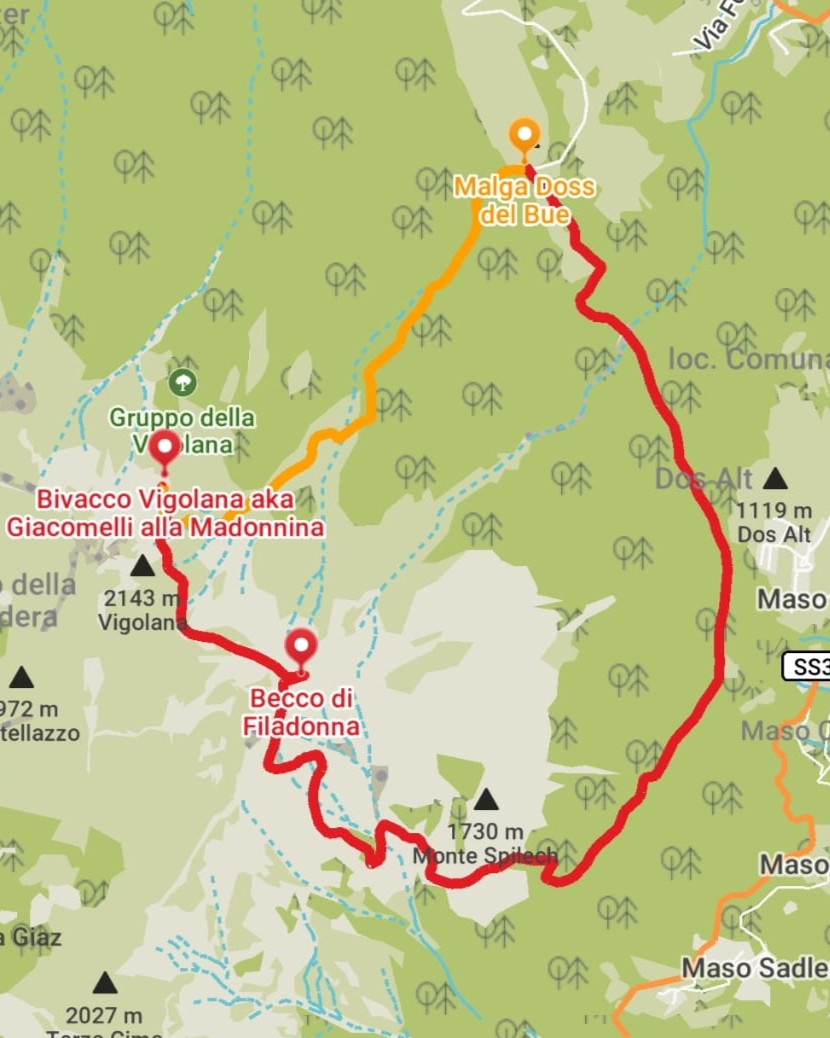
\includegraphics[width=\textwidth]{images/sentiero_mapsMe.jpg}
        \caption{Sentiero su Maps.Me.}
        \label{fig:foto_lunga}
    \end{subfigure}
    \hfill
    % Colonna di destra, allineata in alto
    \begin{subfigure}[t]{0.45\textwidth}
        \centering
        \vspace{0pt} % Forziamo l'allineamento in alto anche qui
        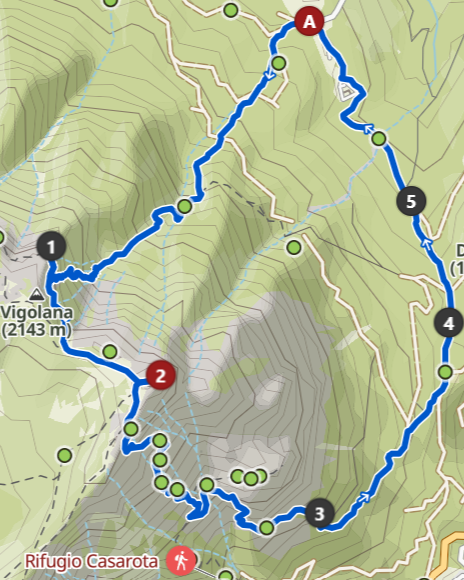
\includegraphics[width=\textwidth]{images/sentiero_komoot.png}
        \caption{Sentiero su Komoot.}
        \label{fig:foto_corta1}
        \vspace{1em} % Aggiunge un po' di spazio tra le due foto
        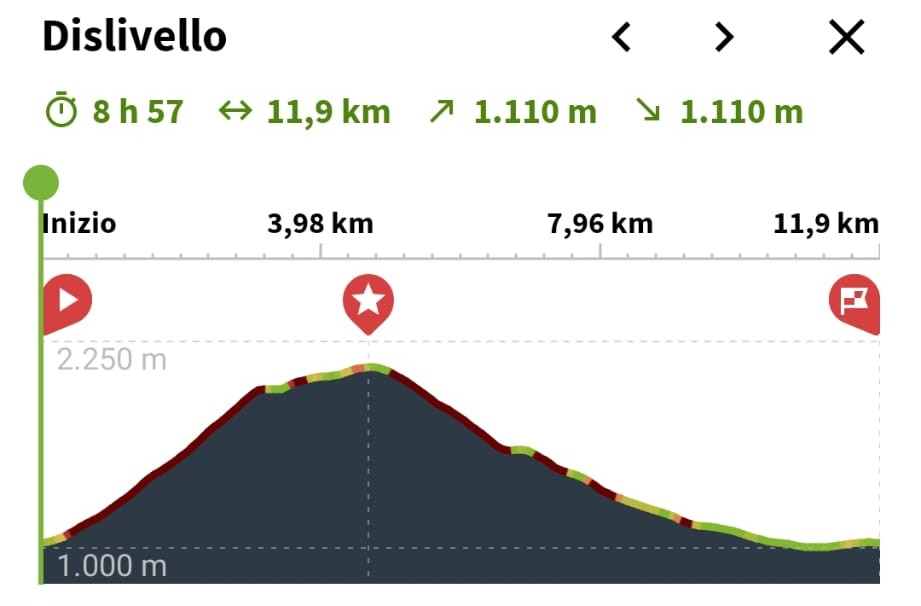
\includegraphics[width=\textwidth]{images/profilo_altimetrico.jpg}
        \caption{Profilo altimetrico del percorso.}
        \label{fig:foto_corta2}
    \end{subfigure}
    % Didascalia generale per l'intera figura
    \caption{Il sentiero e i dettagli del percorso.}
    \label{fig:panoramica_dettagli}
\end{figure}


\section{Non ti scordar di me}
\textbf{\textcolor{BurntOrange}{Ricorda: il bivacco è un bene comune. Il suo futuro dipende dal rispetto e dal senso civico dei visitatori. Usalo con cura e lascialo più pulito di come l'hai trovato.}}


\section{Esperienza personale}
Siamo arrivati al parcheggio verso le 12.00, avevamo due obiettivi principali: scaldare il pane sulla brace e riuscire ad arrivare al bivacco prima che arrivasse da piovere. Spoiler: non siamo riusciti a fare nessuna delle due cose. 

Mentre salivamo abbiamo incontrato il soccorso alpino che ci ha avvisati di prestare attenzione durante la salita perché da lì a poco avrebbe piovuto. Secondo me ce l'hanno gufata: da lì a poco ha iniziato a piovvigginare, fortunatamente i primi 500-600 metri di salita sono all'interno di un bosco, quindi l'acqua che ci prendeva era effettivamente poca. Sicuramente il caldo non aiutava però la prima parte di salita è passata in fretta. I problemi sono arrivati finito questo tratto. È iniziato un sentiero esposto su roccia e per nostra sfortunata ha iniziato a diluviare. È stata la salita più complessa che abbia mai affrontato: scendeva letteralmente un fiume dalla roccia mentre salivamo (a ripensarsi abbiamo fatto una gran cavolata ma siamo stati fortunati). Il bello di tutto ciò non è solo che, appena entrati nel bivacco, ha smesso di piovere ed è tornato il sole, ma anche che, dei 17 presenti quella sera, gli unici ad aver preso l’acqua siamo stati noi cinque. In bivacco abbiamo dormito all'interno in 15, con 2 ragazzi fuori.
Siamo anche riusciti a recuperare un po' d'acqua, in quanto, proseguendo verso la via Ferrata si incontra un tratto di roccia da cui sgorga acqua. Non so se si tratti di una vera fonte o semplicemente di accumuli dovuti alla pioggia: comunque non ci farei troppo affidamento.
Il ritorno il giorno seguente è stato abbastanza semplice, abbiamo raggiunto il Becco di Filadonna e poi siamo tornati a valle.

\section{Alcune foto}

% Sezione Alcune foto

\begin{figure}[htbp!]
    \centering
    % Prima riga: Due foto (QUESTA È LA PRIMA FIGURA)
    \begin{subfigure}[b]{0.45\textwidth}
        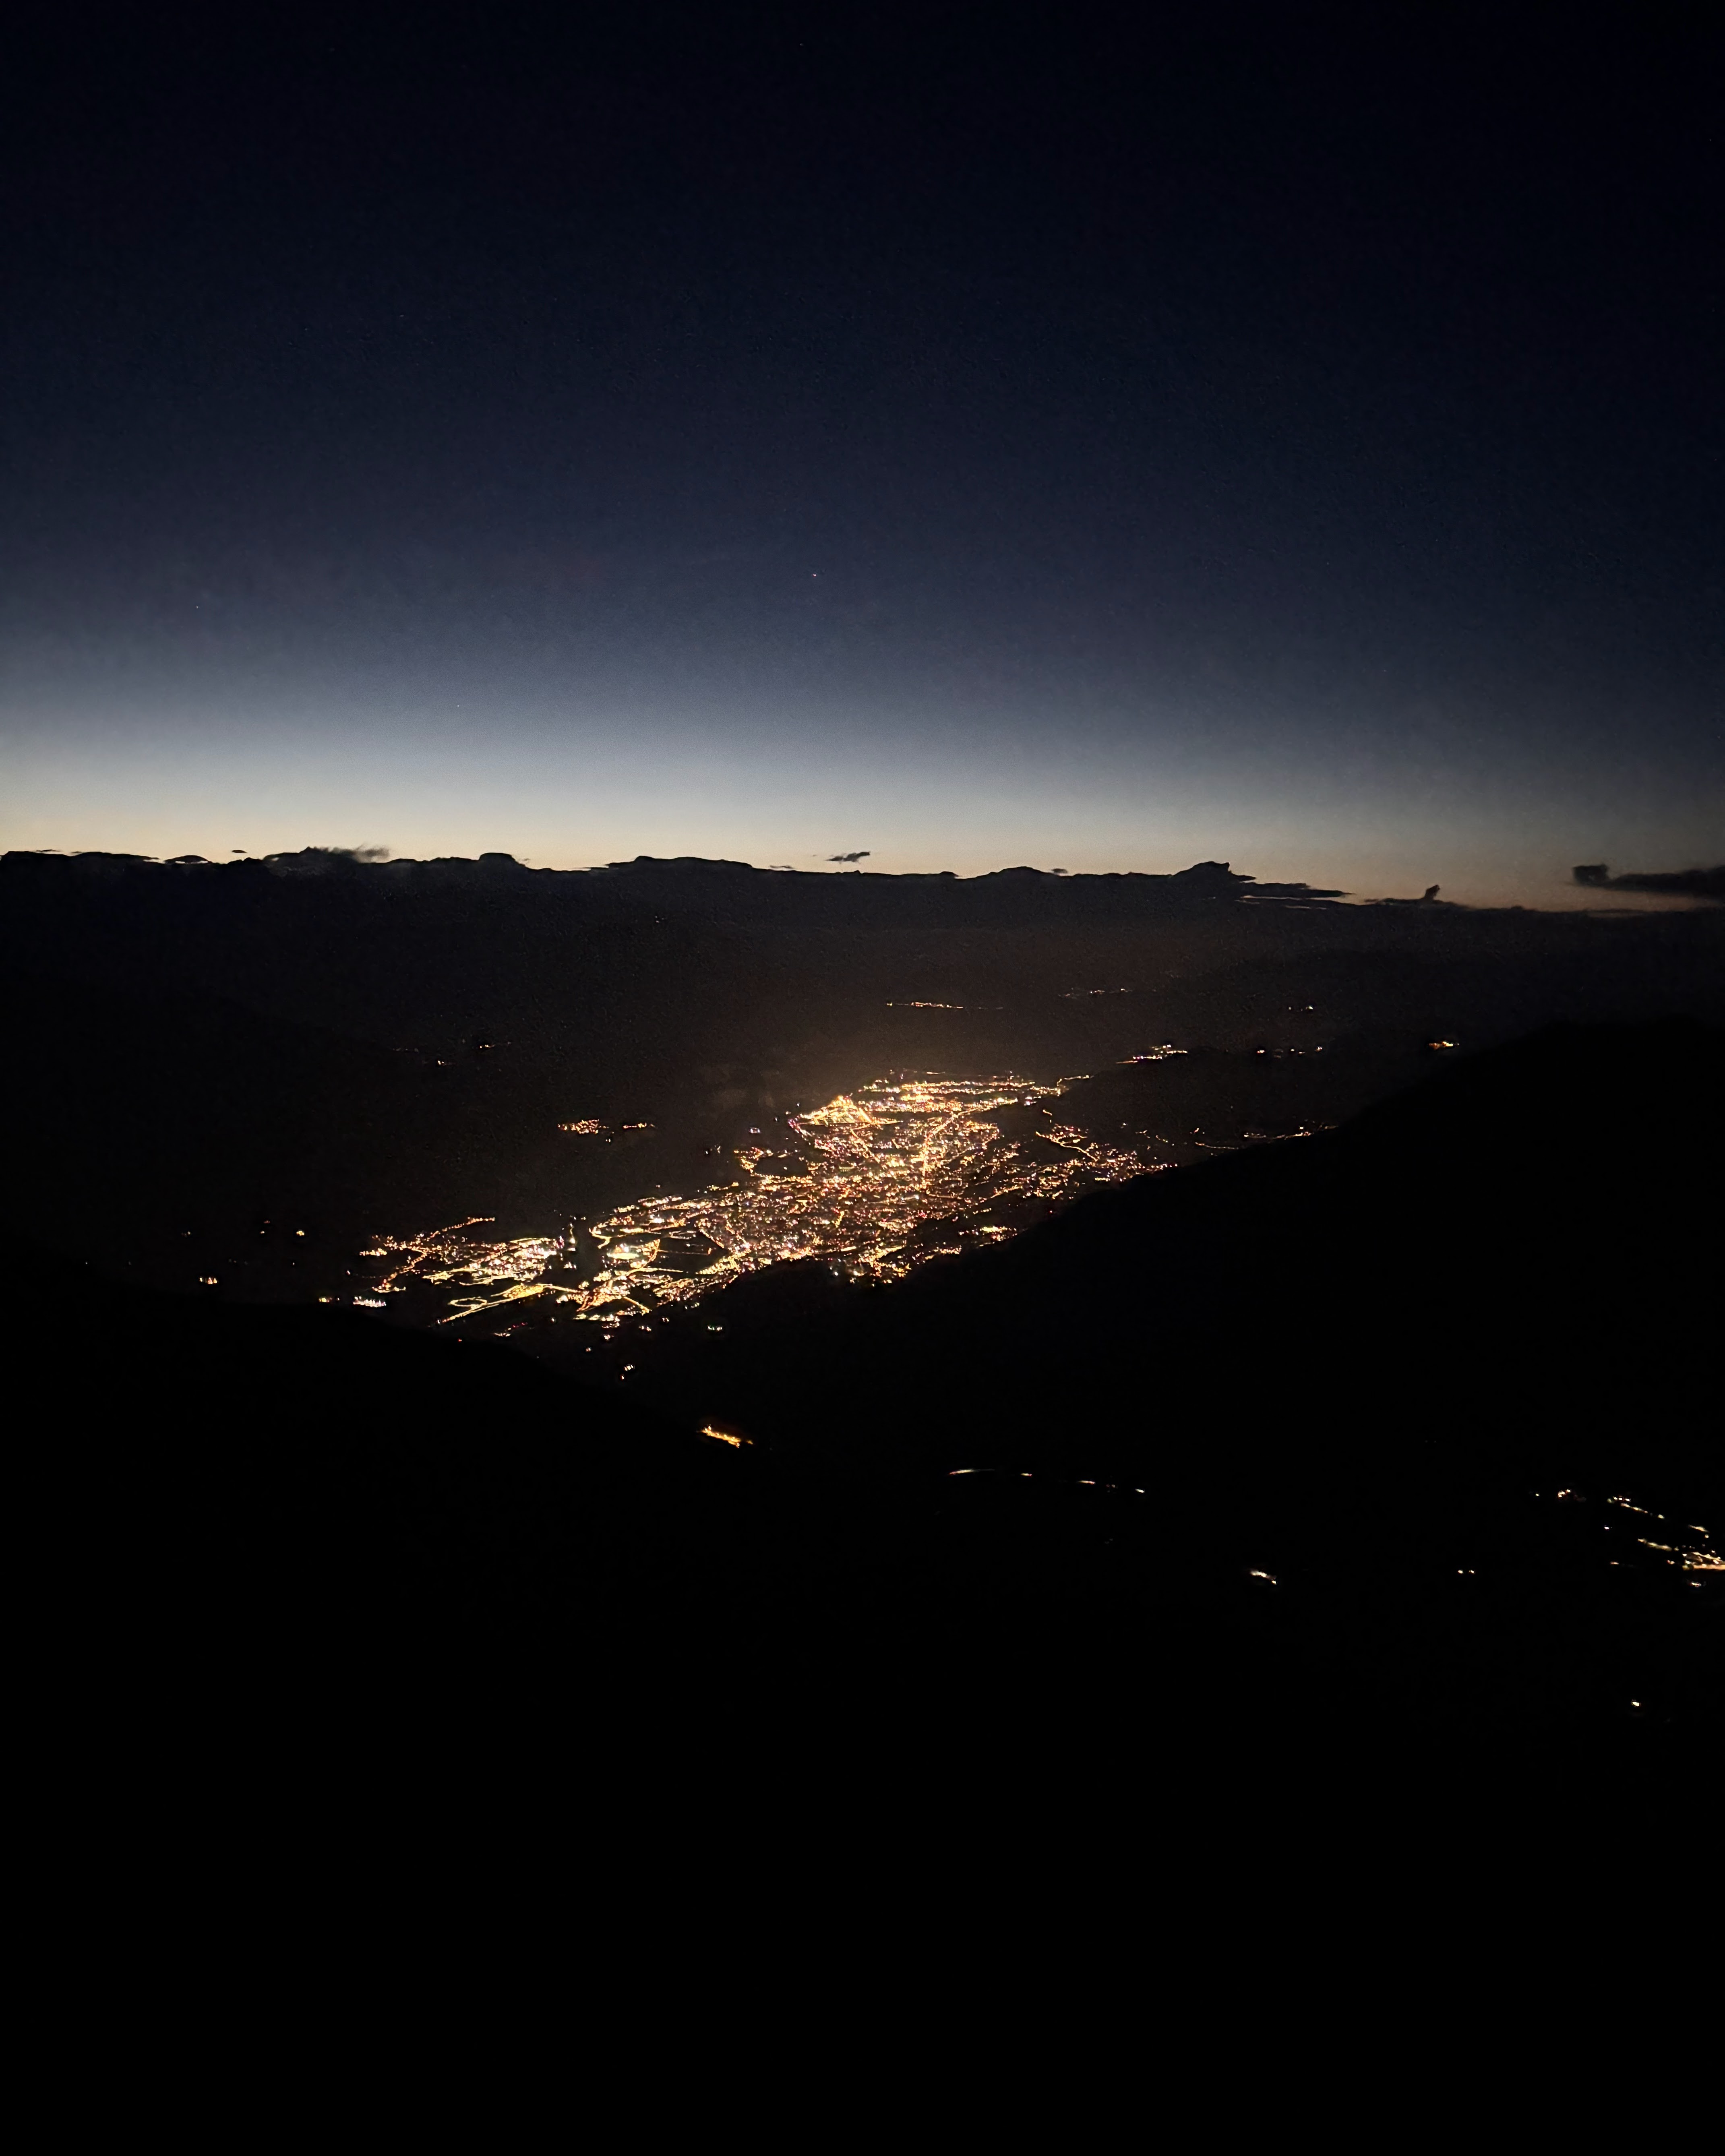
\includegraphics[width=\textwidth]{images/foto_bivaccoNotturna.jpg}
        \caption{Vallata di notte.}
    \end{subfigure}
    \hfill
    \begin{subfigure}[b]{0.45\textwidth}
        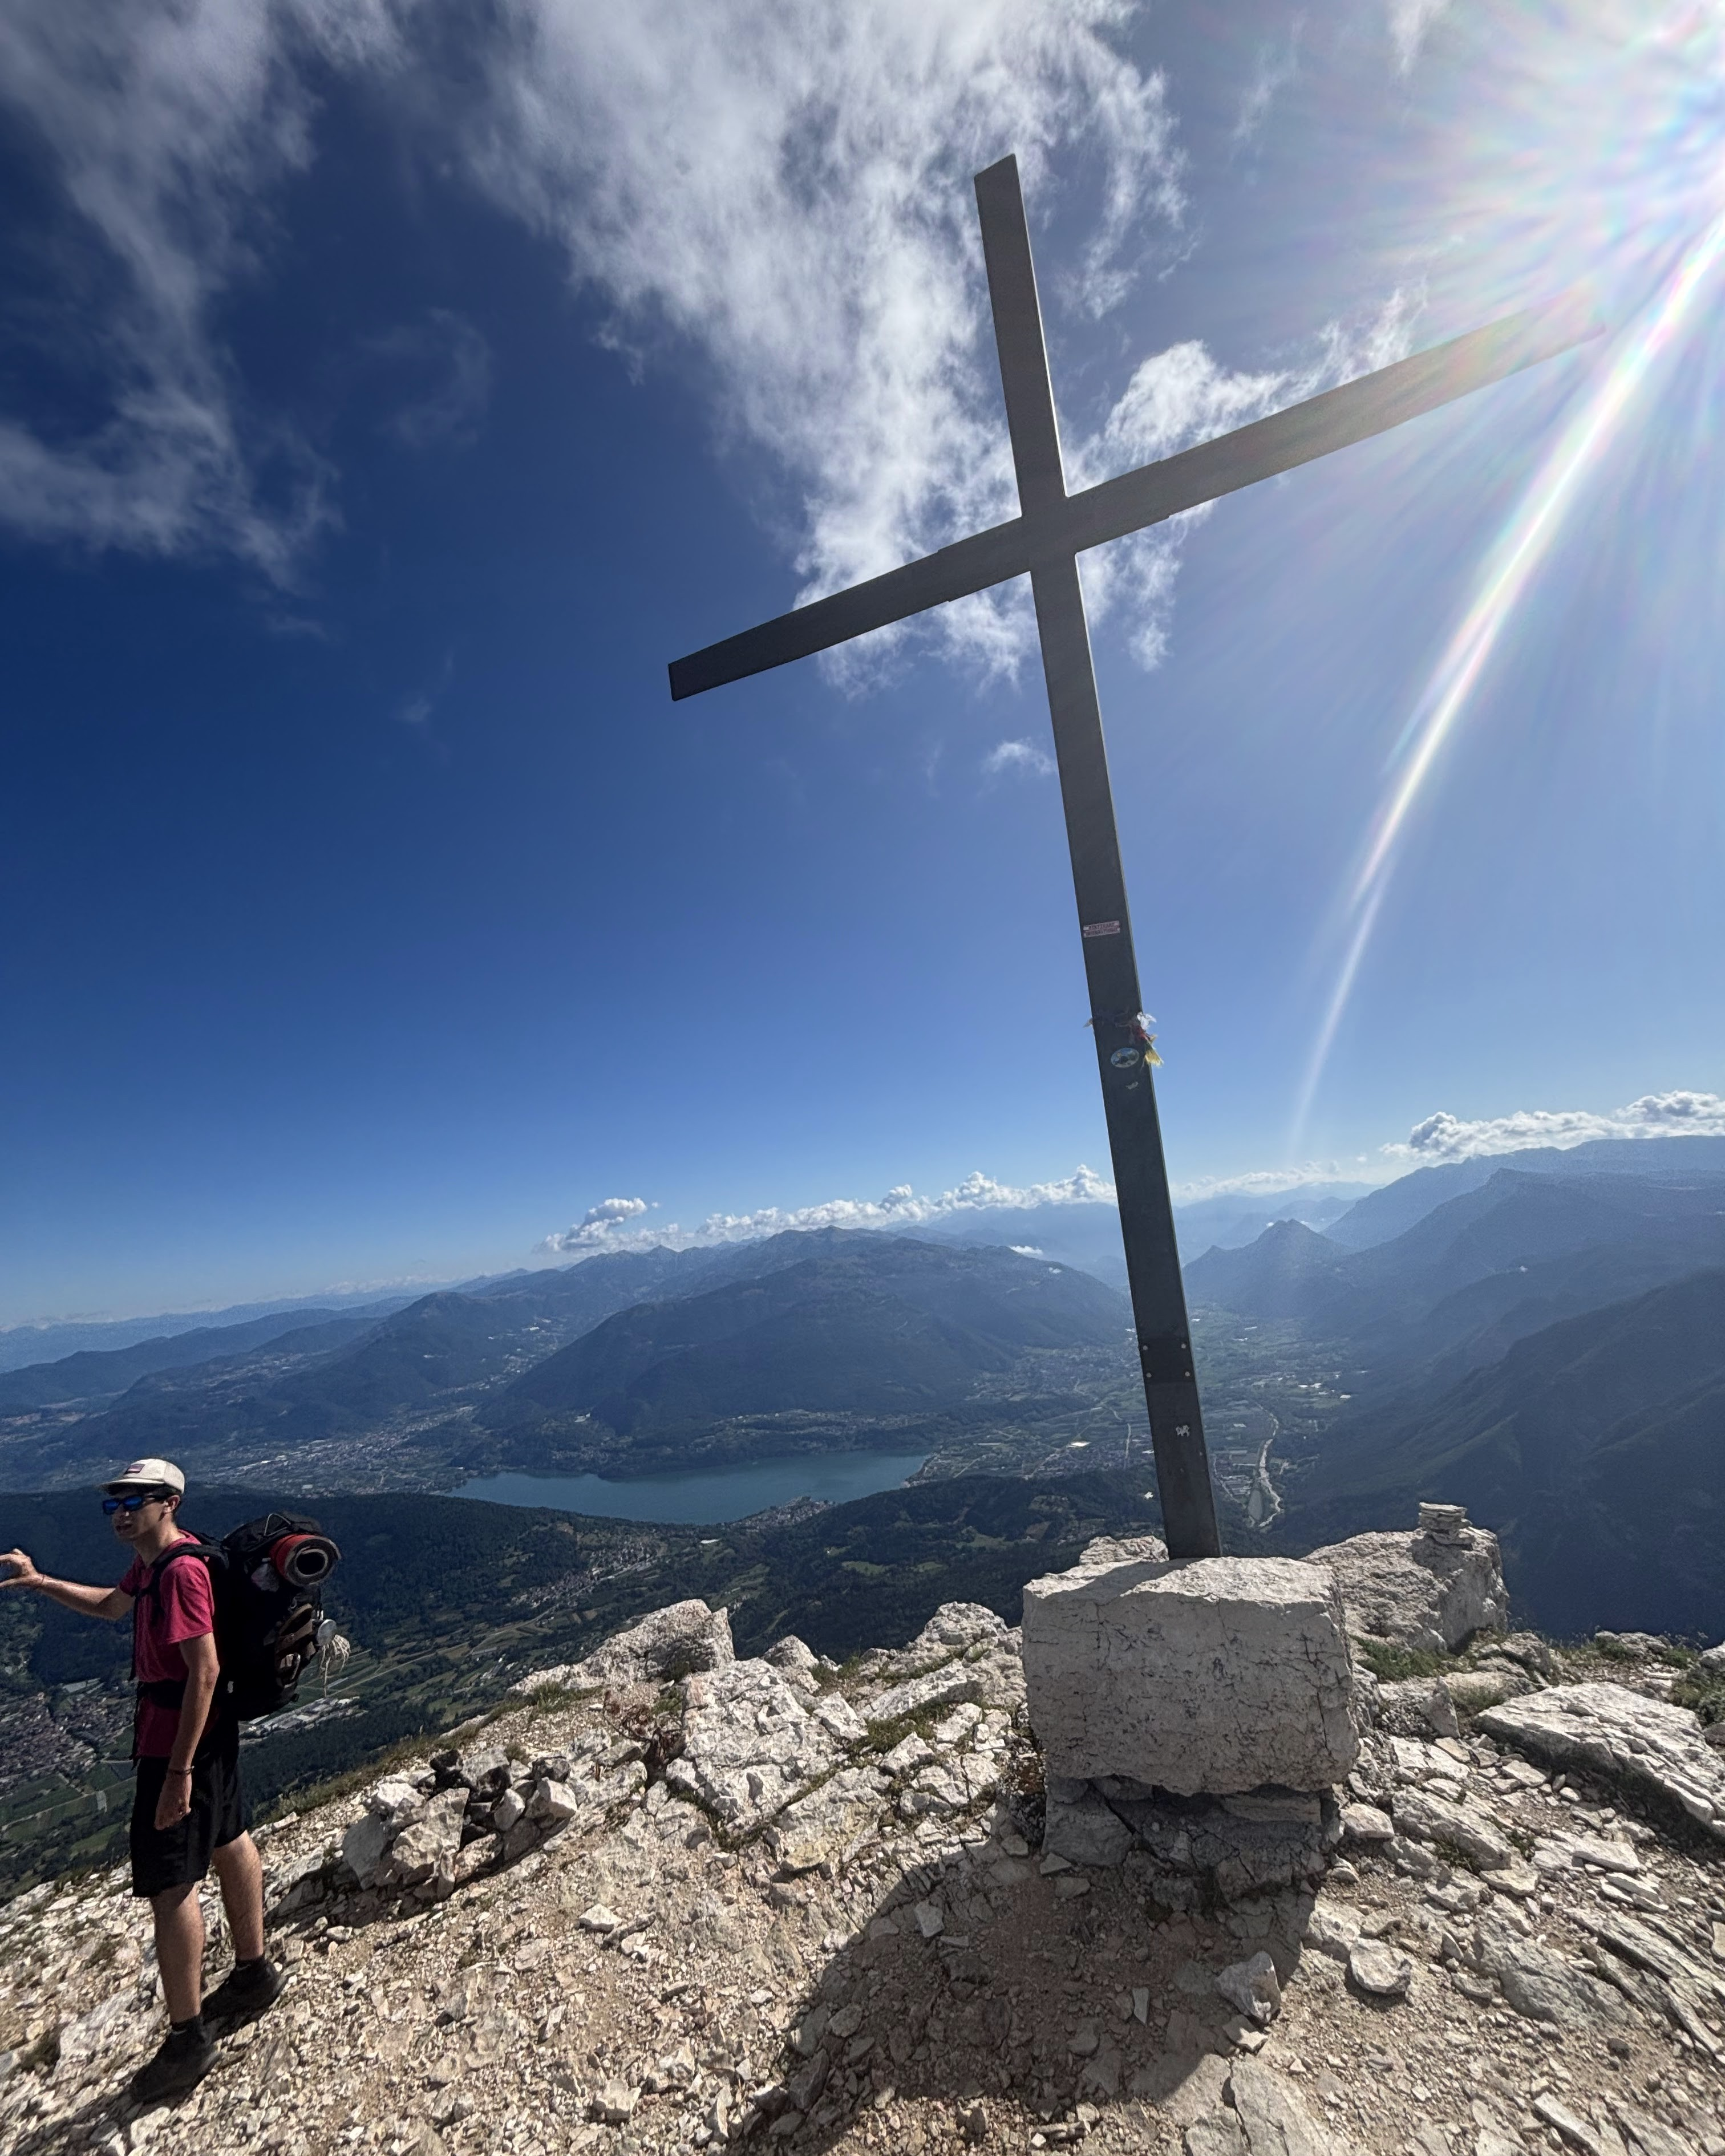
\includegraphics[width=\textwidth]{images/foto_croce.jpg}
        \caption{Becco di Filadonna.}
    \end{subfigure}
  %  \caption{Selezione di fotografie 1.}
\end{figure}

\begin{figure}[htbp!]
    \centering
    % Seconda riga: Tre foto (QUESTA È LA SECONDA FIGURA)
    \begin{subfigure}[b]{0.45\textwidth}
        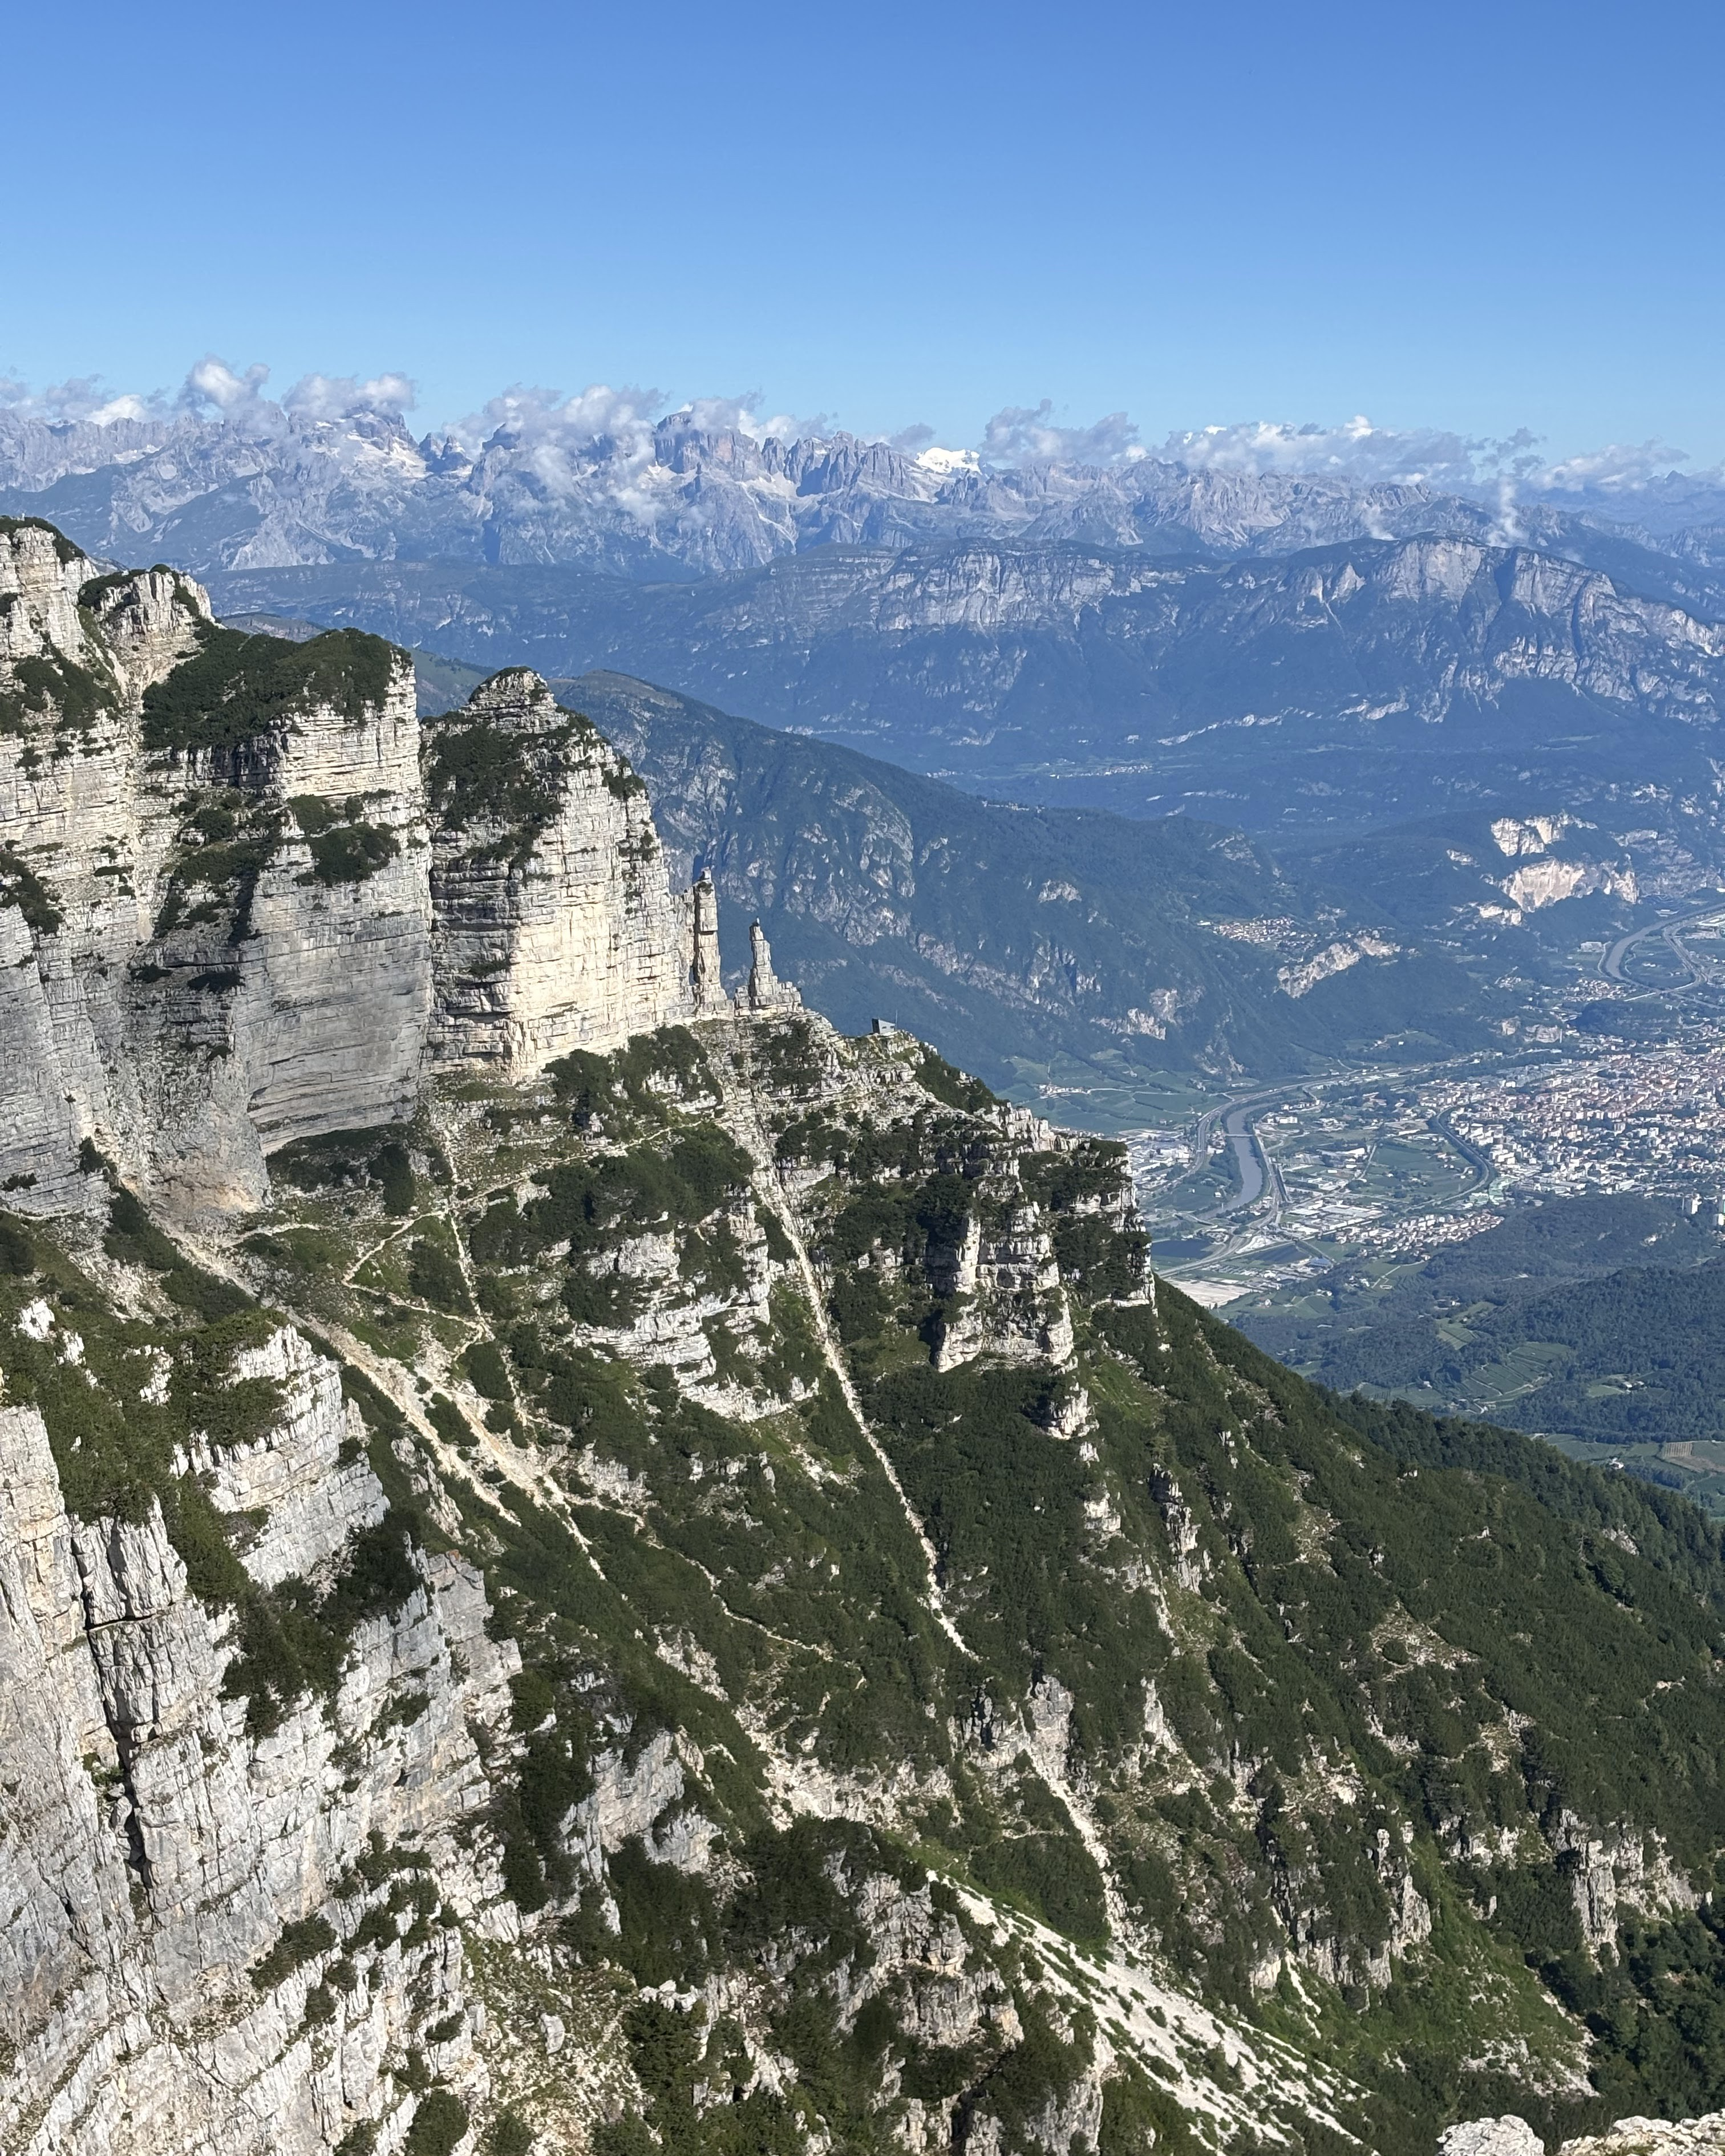
\includegraphics[width=\textwidth]{images/foto_guglie.jpg}
        \caption{Guglie e bivacco dal Becco di Filadonna.}
    \end{subfigure}
    \hfill
    \begin{subfigure}[b]{0.45\textwidth}
        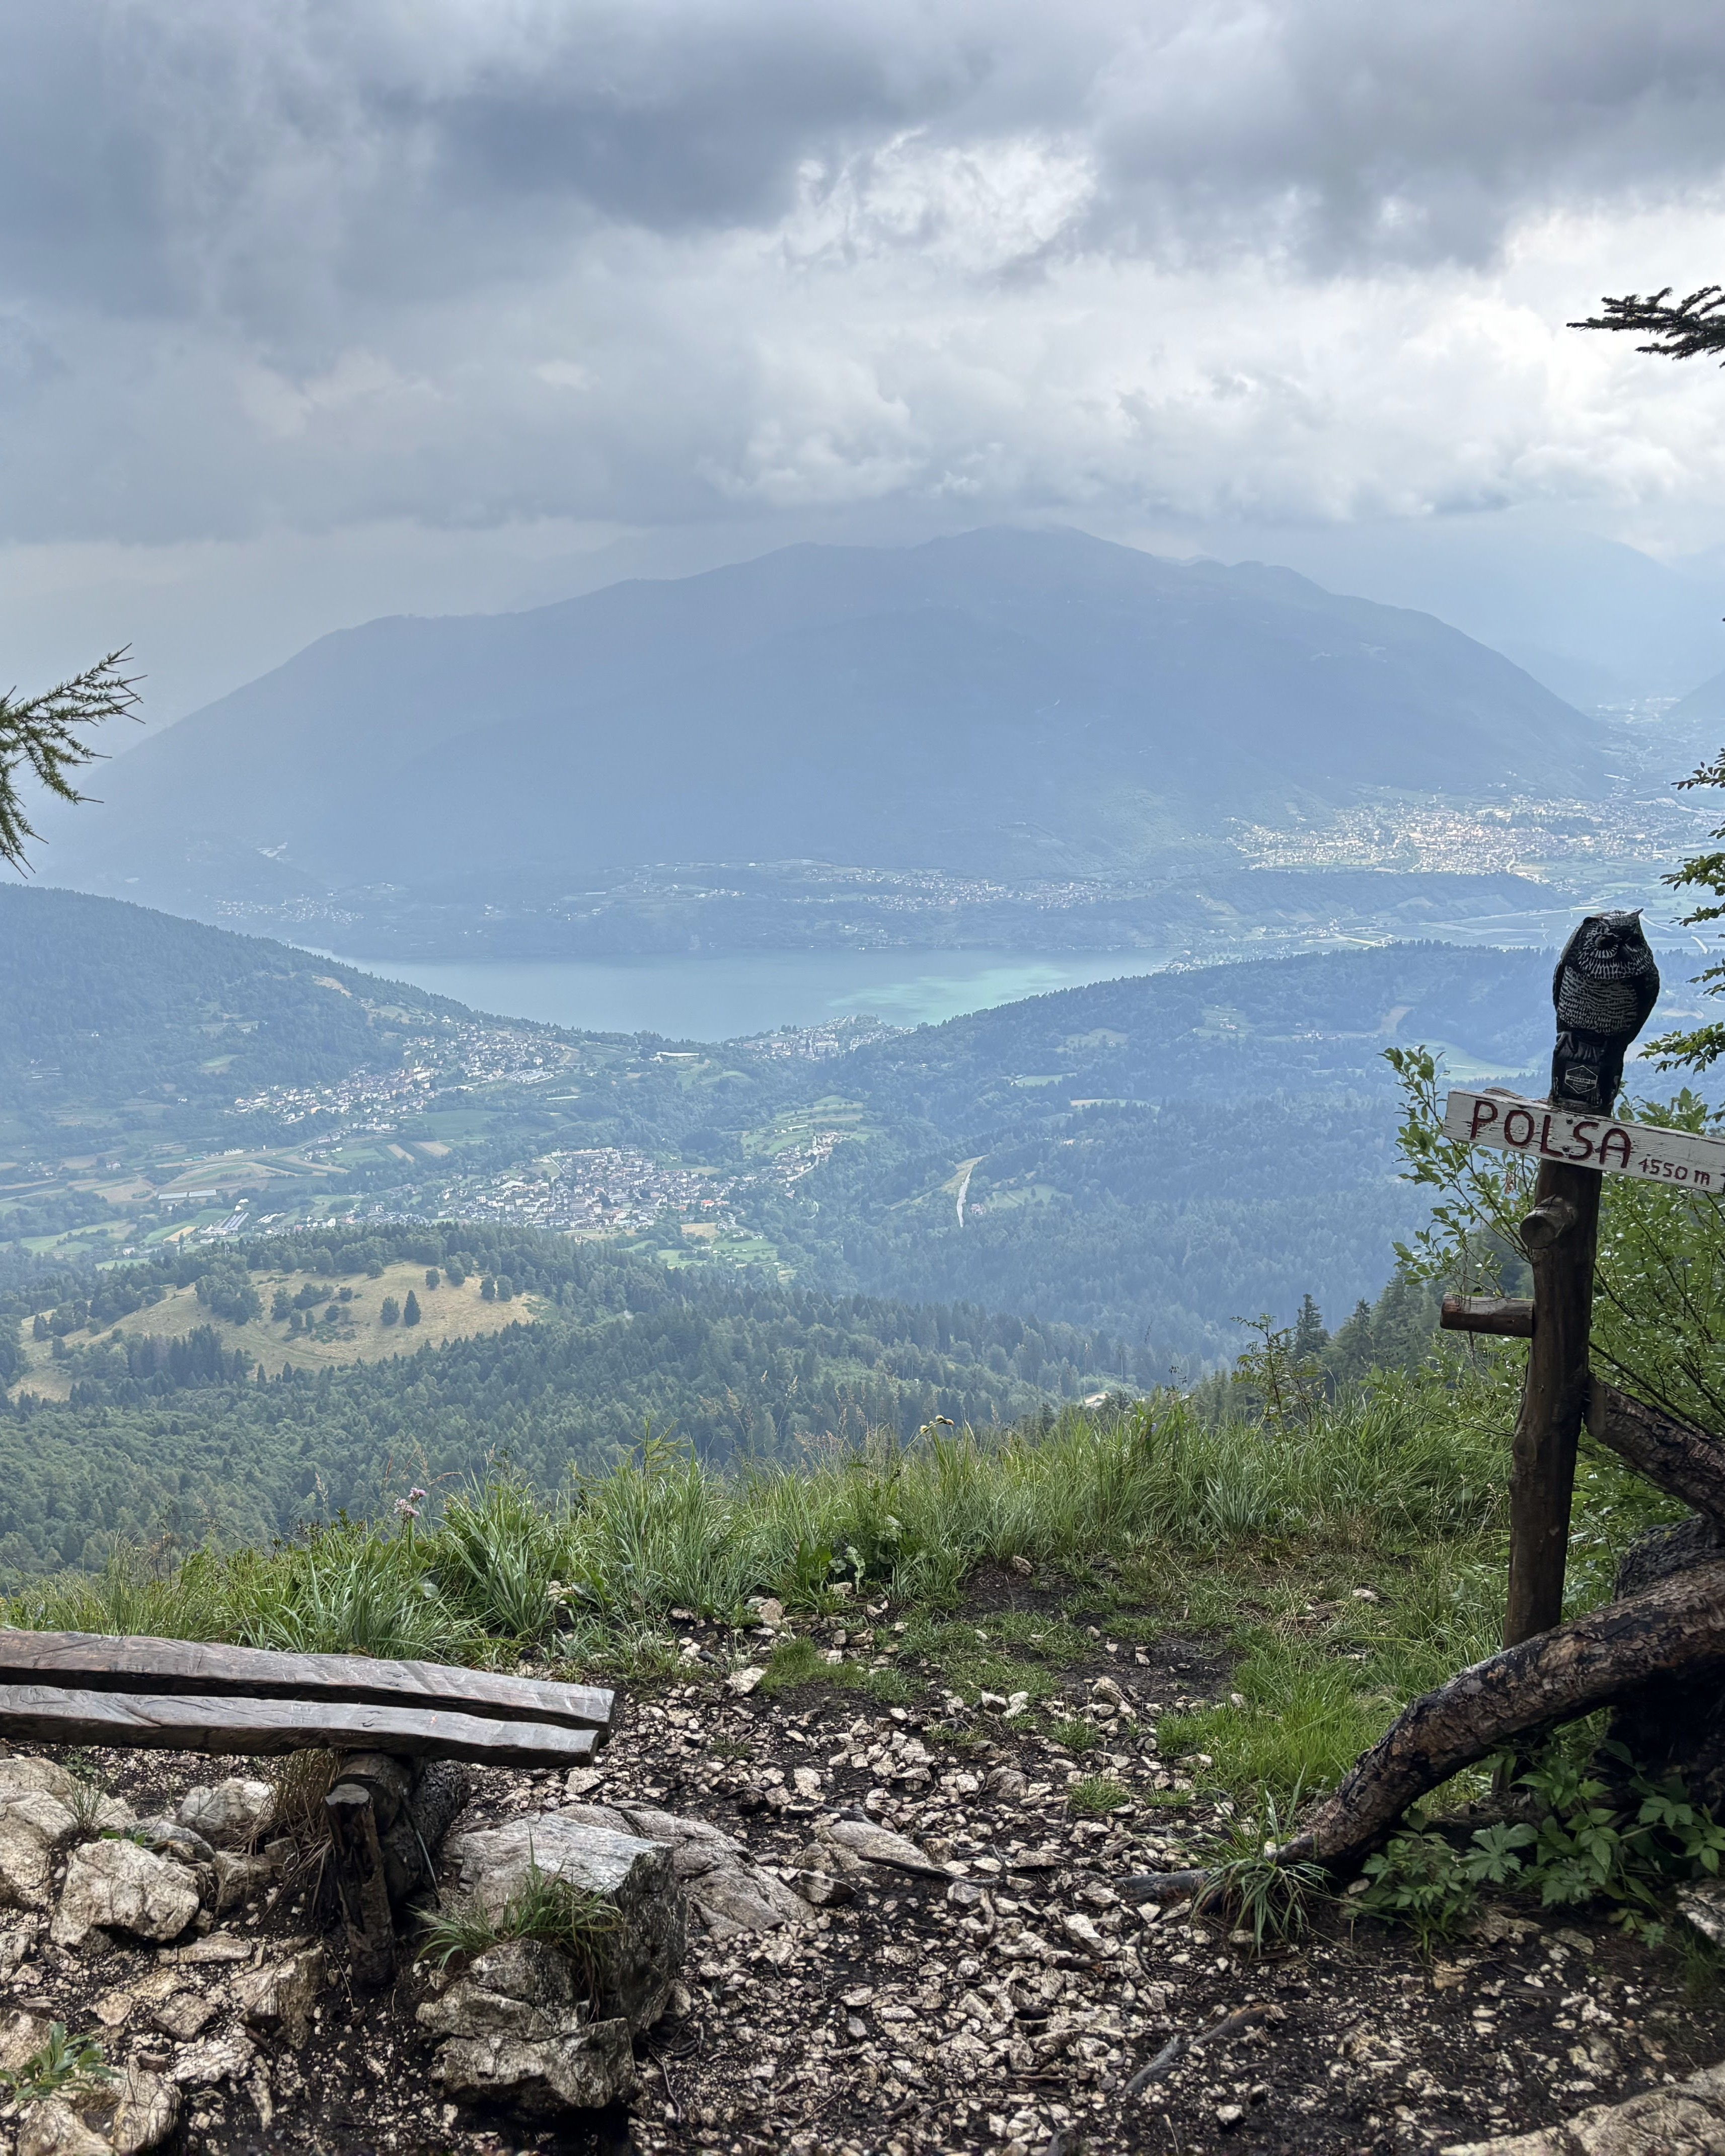
\includegraphics[width=\textwidth]{images/foto_polsa.jpg}
        \caption{Vista dal punto panoramica della Polsa.}
    \end{subfigure}
    \hfill
    
    \vspace{1em}
    
    \begin{subfigure}[b]{\textwidth}
        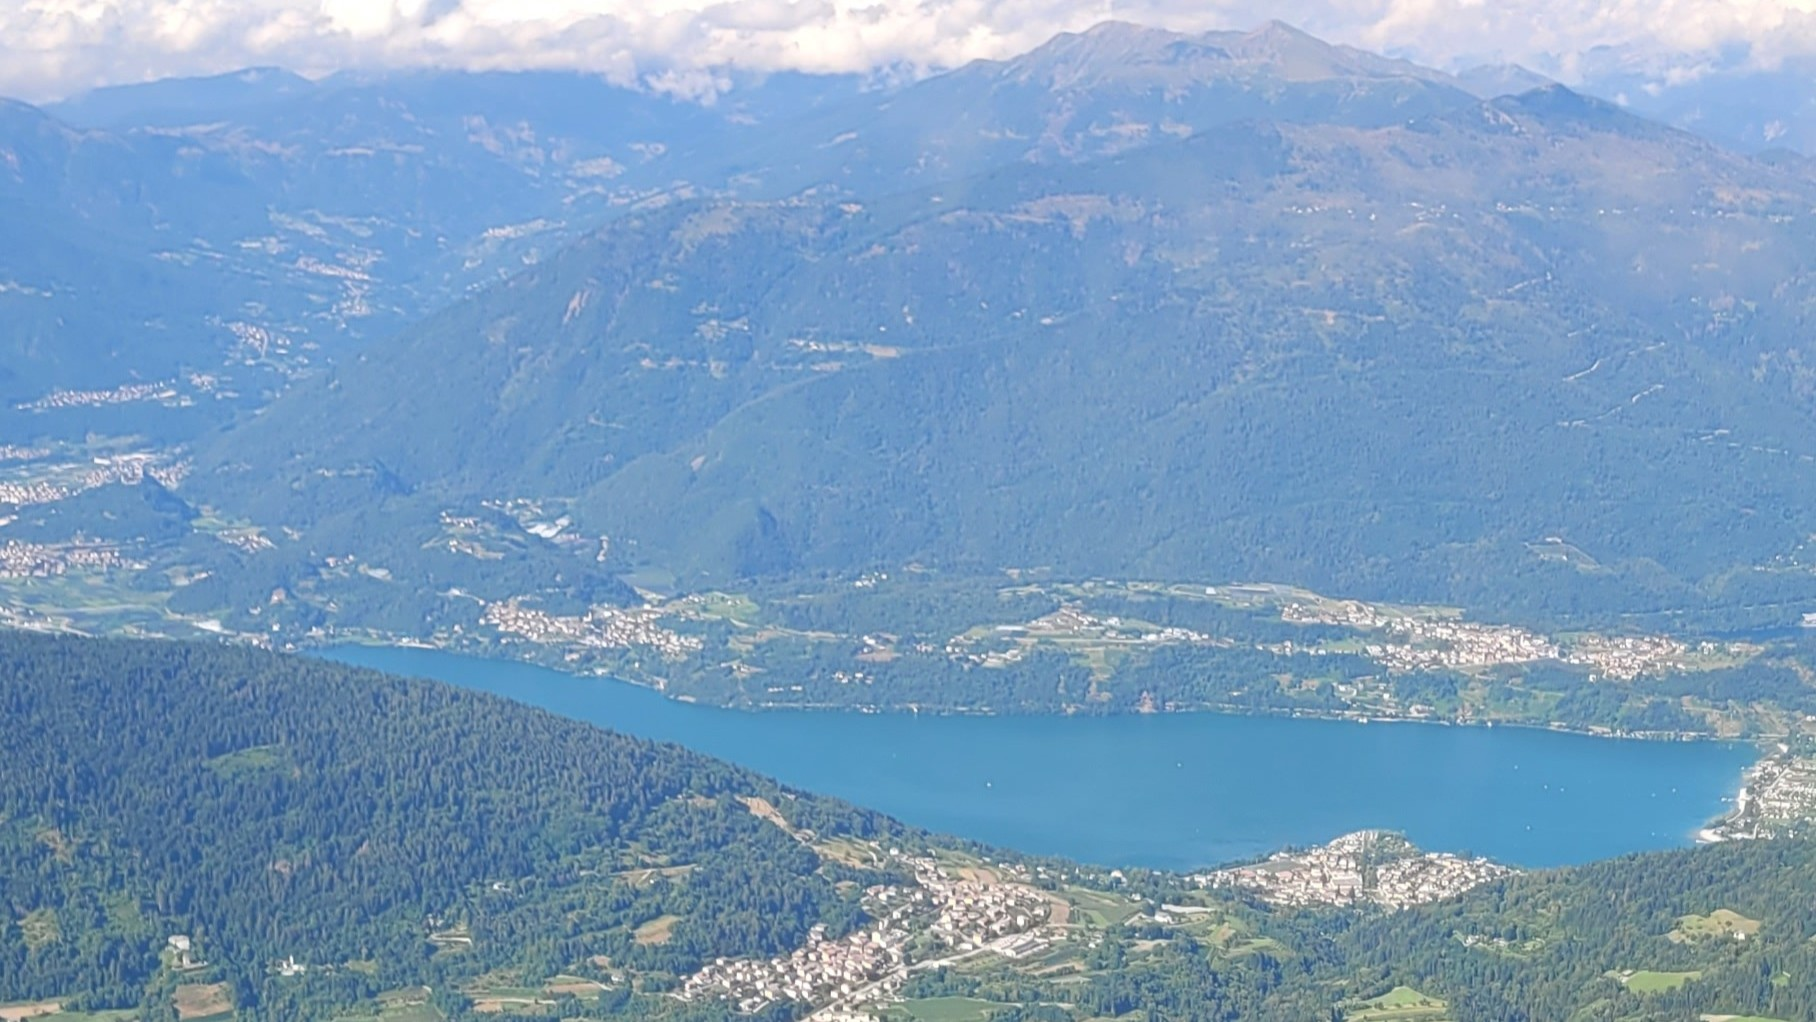
\includegraphics[width=\textwidth]{images/foto_bivacco.jpg}
        \caption{Vista dalla cima.}
    \end{subfigure}
    \caption{Selezione di fotografie del percorso e della vista dal bivacco.}
\end{figure}

\end{document}
